\section*{\centering BAB III\\ HASIL DAN PEMBAHASAN}
\addcontentsline{toc}{section}{BAB III HASIL DAN PEMBAHASAN}

\lipsum[1]

\begin{figure}[H]
    \centering
    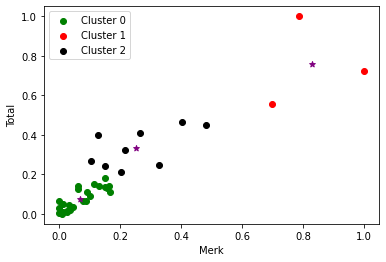
\includegraphics[scale=.5]{Image/plot1.png}
    \caption{Caption gambar 1}
    \label{fig:my_label3}
\end{figure}

\lipsum[2]

\lipsum[3]

\lipsum[4]

\lipsum[5]
\begin{table}[h]
\begin{center} {\footnotesize

\begin{tabular}{lll}
\hline
 \multicolumn{1}{c}{Cluster 0} & \multicolumn{1}{c}{Cluster 1} & \multicolumn{1}{c}{Cluster 2}\\
\hline
    sosis, saus, tomat  &  mie, ayam, sayur  & es, kopi	\\[.2ex]
    es, buah  &  nasi, ayam, pedas  &  ayam, roti, es  \\[.2ex] 
    es, roti, cokelat &  nasi, mie, kopi  &   nasi, ayam \\[.2ex] 
    daging, sayur &    &  mie, ayam, bakso \\[.2ex] 
    ikan, tepung, pedas &    & nasi, mie, sayur	 \\[.2ex] 
    nasi, seafood, pedas &    & tepung, selai\\[.2ex] 
    mie, saus, roti &    & es, kopi, cokelat  \\[.2ex] 
    tepung, cokelat	 &    & es, teh \\[.2ex] 
    lontong, sayur, kacang &    & bakso, kuah, mie\\[.2ex] 
    ayam, kambing, kacang &    &    \\[.2ex] 
    babi, kacang &    &    \\[.2ex] 
    ayam, kuah &    &    \\[.2ex] 
    mie, seafood, nasi &    &    \\[.2ex] 
    bebek, tepung, pedas &    &    \\[.2ex] 
    nasi, ayam, sayur &    &    \\[.2ex] 
    es, roti &    &    \\[.2ex] 
    nasi, sayur, pedas &    &    \\[.2ex] 
    ayam, sapi, kuah &    &    \\[.2ex]
    buah, pedas, kacang &    &    \\[.2ex]
    tahu, sosis, kacang &    &    \\[.2ex]
    ikan, pedas &    &    \\[.2ex]
    sayur, tepung &    &    \\[.2ex]
    susu, teh &    &    \\[.2ex]
    daging, pedas &    &    \\[.2ex]
    kulit, tepung, daging &    &    \\[.2ex]
\hline
\end{tabular}
}
\end{center}
\caption{Caption tabel 1}
\label{turns}
\end{table}

\lipsum[6]